\documentclass[12pt]{article}
\usepackage{graphicx}
\usepackage[utf8]{inputenc}
\usepackage[T1]{fontenc}
\usepackage{amsmath, pgfplots, pgf, pdfpages, amsfonts, amssymb, stmaryrd, enumitem,graphicx, algpseudocode, setspace, listings, courier, color, caption, centernot, hyperref, lstautogobble, zi4, mathtools, lmodern, colortbl, array, multicol, fancyhdr, lastpage, booktabs, biblatex, svg, pdflscape, multirow, longtable, esint, tikz}
\usepackage{amsmath} % for \dfrac
\usepackage{bm}
\usepackage{physics}
\usepackage{tikz,pgfplots}
\usetikzlibrary{angles,quotes} % for pic (angle labels)
\usetikzlibrary{calc}
\usetikzlibrary{decorations.markings}
\tikzset{>=latex} % for LaTeX arrow head

\usepackage{xcolor}
\colorlet{Ecol}{orange!90!black}
\colorlet{EcolFL}{orange!80!black}
\colorlet{veccol}{green!45!black}
\colorlet{EFcol}{red!60!black}
\tikzstyle{charged}=[top color=blue!20,bottom color=blue!40,shading angle=10]
\tikzstyle{darkcharged}=[very thin,top color=blue!60,bottom color=blue!80,shading angle=10]
\tikzstyle{charge+}=[very thin,top color=red!80,bottom color=red!80!black,shading angle=-5]
\tikzstyle{charge-}=[very thin,top color=blue!50,bottom color=blue!70!white!90!black,shading angle=10]
\tikzstyle{gauss surf}=[green!40!black,top color=green!2,bottom color=green!80!black!70,shading angle=5,fill opacity=0.5]
\tikzstyle{gauss lid}=[gauss surf,middle color=green!80!black!20,shading angle=40,fill opacity=0.6]
\tikzstyle{gauss dark}=[green!50!black,fill=green!60!black!70,fill opacity=0.8]
\tikzstyle{gauss line}=[green!40!black]
\tikzstyle{gauss dashed line}=[green!60!black!80,dashed,line width=0.2]
\tikzstyle{EField}=[->,thick,Ecol]
\tikzstyle{vector}=[->,thick,veccol]
\tikzstyle{normalvec}=[->,thick,blue!80!black!80]
\tikzstyle{EFieldLine}=[thick,EcolFL,decoration={markings,
          mark=at position 0.5 with {\arrow{latex}}},
          postaction={decorate}]
\tikzstyle{measure}=[fill=white,midway,outer sep=2]
\def\L{8}
\def\W{0.25}
\def\N{14}
\usepackage{newtxtext,newtxmath}
\usepackage{pgfplots}
\pgfplotsset{compat=1.18}
\usepackage[a4paper, left=1.25in, right=1in, top=1in, bottom=1in, nomarginpar]{geometry}
\usepackage[framemethod=TikZ]{mdframed}
\newmdenv[%
    skipabove=1em, % space above the frame
    skipbelow=1em, % space below the frame
    linewidth=1pt, % width of the frame lines
    linecolor=gray!40, % color of the frame lines
    backgroundcolor=gray!10, % background color inside the frame
    roundcorner=3pt, % radius of the rounded corners
    innerleftmargin=1em, % margin within the frame at the left
    innerrightmargin=1em, % margin within the frame at the right
    innertopmargin=0.5em, % margin within the frame at the top
    innerbottommargin=0.5em % margin within the frame at the bottom
]{qframe}

\newenvironment{q}
{
    \begin{qframe}
    \noindent\textit{\textbf{Problem Statement:}}
    \par\smallskip
}
{
    \end{qframe}
}


\begin{document}

\tableofcontents
\listoffigures
\newpage
\section*{Question 1}
\addcontentsline{toc}{section}{Question 1}
\begin{q}
1) What are the fundamental equations of electrostatics? Explain their meaning. Give the name and unit of each term seen in the equations.
\end{q}

Consider a region in Euclidean space, \(\mathbb{R}^3\), endowed with a vector field \(\vec{E}(\vec{r})\), representing the electric field at a point \(\vec{r}\), and a scalar field \(\rho(\vec{r})\), denoting the volume charge density at \(\vec{r}\). The electrostatic regime is characterized by the absence of time-varying magnetic fields, which allows for a simplification of Maxwell's equations. Within this framework, we examine the following equations:

1. \textit{Gauss's Law for Electrostatics}: The divergence of the electric field \(\vec{E}\) is proportional to the local charge density \(\rho\), scaled by the permittivity of free space \(\varepsilon_0\), a fundamental constant. Mathematically, this is expressed as:
   \[
   \nabla \cdot \vec{E} = \frac{\rho}{\varepsilon_0}
   \]

This equation elucidates the principle that electric charge acts as the source or sink of electric field lines. In the language of differential geometry, the divergence operator here acts on the vector field \(\vec{E}\), yielding a scalar field that describes the density of the field's sources.

2. \textit{Electrostatics and Faraday's Law}: In the static case, Faraday's law asserts that the electric field \(\vec{E}\) is irrotational, leading to:
   \[
   \nabla \times \vec{E} = \vec{0}
   \]

This curl-free condition signifies that the electric field can be expressed as the gradient of a scalar potential \(V\), thus \(\vec{E} = -\nabla V\). The negative sign reflects the convention that electric field lines point in the direction of decreasing potential.

3. \textit{Coulomb's Law}: While not a Maxwell equation, Coulomb's law provides the foundational pairwise interaction between point charges in vacuum. For charges \(q_1\) and \(q_2\) separated by a distance \(r\), the electric field generated by \(q_1\) at the location of \(q_2\) is given by:
   \[
   \vec{E} = \frac{q_1}{4\pi\varepsilon_0 r^2} \hat{r}
   \]
   where \(\hat{r}\) is a unit vector pointing from \(q_1\) to \(q_2\). This expression encapsulates the inverse-square law and the principle of superposition inherent in electrostatic interactions.

4. \textit{The Scalar Potential and the Electric Field}: The relation between the electric field and the electric potential \(V\) is succinctly captured by:
   \[
   \vec{E} = -\nabla V
   \]
   This equation defines the electric field as the gradient of the scalar potential \(V\), emphasizing the conservative nature of electrostatic fields.

Each term in these equations carries specific physical dimensions: \([\vec{E}]\) denotes the electric field with units of volts per meter (V/m), \([\rho]\) the charge density with units of coulombs per cubic meter (C/m\(^3\)), \([\varepsilon_0]\) the permittivity of free space with units of farads per meter (F/m), and \([V]\) the electric potential with units of volts (V). These dimensions underpin the quantifiable nature of electrostatic phenomena.

\newpage
\section*{Question 2}
\addcontentsline{toc}{section}{Question 2}
\begin{q}
2) A spherical cloud of radius \(a\) has a volume charge of density \(\rho_V=1 / r \mathrm{C} / \mathrm{m}^3\). Find and draw the electric field strength at all points.
\end{q}


\textbf{Inside the Spherical Cloud (\(r \leq a\)).}


Let us consider a Gaussian surface, \(S\), a sphere of radius \(r\) where \(r \leq a\), concentric with the charge distribution. The symmetry of the problem dictates that the electric field, \(E\), at any point on \(S\) is radial and its magnitude depends solely on \(r\). Gauss's law, \(\oiint_S \vec{E} \cdot d\vec{A} = \frac{Q_{\text{enc}}}{\varepsilon_0}\), relates the electric flux through \(S\) to the charge enclosed, \(Q_{\text{enc}}\), by the surface.

Given \(\rho_V = \frac{1}{r}\), the charge enclosed by the Gaussian surface is determined by integrating the charge density over the volume enclosed by \(S\):
\[
Q_{\text{enc}} = \int_V \rho_V dV = \int_0^r 4\pi r'^2 \frac{1}{r'} dr' = 4\pi \int_0^r r' dr' = 2\pi r^2.
\]
Applying Gauss's law yields the electric field as a function of \(r\) for \(r \leq a\):
\[
E \cdot 4\pi r^2 = \frac{2\pi r^2}{\varepsilon_0} \implies E(r) = \frac{r}{2\varepsilon_0}.
\]

\textbf{Outside the Spherical Cloud (\(r > a\)).}


For \(r > a\), the entire charge within the cloud contributes to the electric field at \(r\). The total charge, \(Q\), is obtained by integrating the charge density over the entire volume of the cloud:
\[
Q = \int_0^a 4\pi r^2 \frac{1}{r} dr = 4\pi \int_0^a r dr = 2\pi a^2.
\]
And
\[
E \cdot 4\pi r^2 = \frac{2\pi a^2}{\varepsilon_0} \implies E(r) = \frac{a^2}{2\varepsilon_0 r^2}.
\]

So, the electric field generated by the spherical cloud is thus expressed by:\[
E(r) = \begin{cases}
\frac{r}{2\varepsilon_0}, & \text{for } r \leq a, \\
\frac{a^2}{2\varepsilon_0 r^2}, & \text{for } r > a.
\end{cases}
\]


\begin{figure}[ht!]
\centering
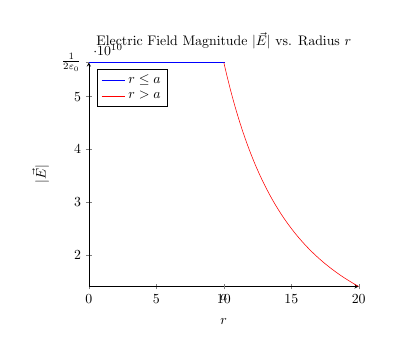
\begin{tikzpicture}[scale=0.5]
\begin{axis}[
    axis lines = left,
    xlabel = \(r\),
    ylabel = {\(|\vec{E}|\)},
    domain=0:2*10, % This sets the overall domain for the plot.
    samples=1000,
    legend pos=north west,
    title={Electric Field Magnitude \(|\vec{E}|\) vs. Radius \(r\)},
    yticklabel style={/pgf/number format/fixed},
    extra y ticks={1/(2*8.854e-12)},
    extra y tick labels={\(\frac{1}{2\varepsilon_0}\)},
    extra x ticks={10},
    extra x tick labels={\(a\)},
]

% Inside the spherical cloud
\addplot[blue, domain=0:10] {1/(2*8.854e-12)};
\addlegendentry{\(r \leq a\)}

% Outside the spherical cloud
\addplot[red, domain=10:20] {100/(2*8.854e-12*x^2)};
\addlegendentry{\(r > a\)}

\end{axis}
\end{tikzpicture}
\caption{A plot of the electric field magnitude \(|\vec{E}|\) as a function of the radius \(r\)}
\label{fig:EfieldPlot}
\end{figure}



\newpage
\section*{Question 3}
\addcontentsline{toc}{section}{Question 3}
\begin{q}
3) Determine the electric field intensity \(\vec{E}\) and the potential \(V\) at point \(P\), show that \(\vec{E}=-\nabla V\).
\end{q}

\begin{figure}[ht!]
\centering
\tikzset{every picture/.style={line width=0.75pt}} %set default line width to 0.75pt        
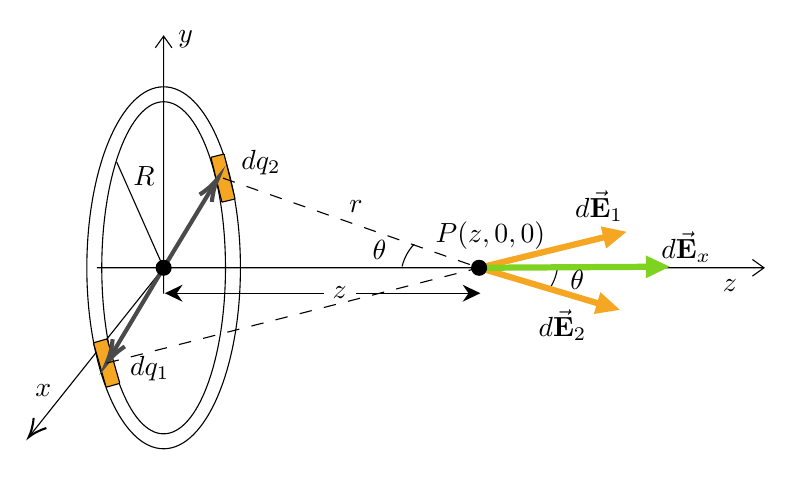
\begin{tikzpicture}[x=0.75pt,y=0.75pt,yscale=-1,xscale=1, scale=0.8]
%uncomment if require: \path (0,444); %set diagram left start at 0, and has height of 444

%Shape: Arc [id:dp796341774674139] 
\draw  [draw opacity=0] (262.37,163.17) .. controls (263.64,157.97) and (266.21,153.41) .. (269.66,149.76) -- (291.5,170.33) -- cycle ; \draw   (262.37,163.17) .. controls (263.64,157.97) and (266.21,153.41) .. (269.66,149.76) ;
%Shape: Arc [id:dp46939057871839585] 
\draw  [draw opacity=0] (356.12,162.23) .. controls (355.71,167.57) and (353.93,172.5) .. (351.13,176.67) -- (326.2,159.96) -- cycle ; \draw   (356.12,162.23) .. controls (355.71,167.57) and (353.93,172.5) .. (351.13,176.67) ;
%Straight Lines [id:da14186153692575143] 
\draw [color={rgb, 255:red, 245; green, 166; blue, 35 }  ,draw opacity=1 ][line width=2.25]    (308.75,164) -- (388.71,187.9) ;
\draw [shift={(393.5,189.33)}, rotate = 196.64] [fill={rgb, 255:red, 245; green, 166; blue, 35 }  ,fill opacity=1 ][line width=0.08]  [draw opacity=0] (14.29,-6.86) -- (0,0) -- (14.29,6.86) -- cycle    ;
%Straight Lines [id:da24228394907316253] 
\draw [color={rgb, 255:red, 245; green, 166; blue, 35 }  ,draw opacity=1 ][line width=2.25]    (308.75,164) -- (392.64,143.52) ;
\draw [shift={(397.5,142.33)}, rotate = 526.28] [fill={rgb, 255:red, 245; green, 166; blue, 35 }  ,fill opacity=1 ][line width=0.08]  [draw opacity=0] (14.29,-6.86) -- (0,0) -- (14.29,6.86) -- cycle    ;
%Shape: Donut [id:dp6846402688267834] 
\draw   (81.5,164) .. controls (81.5,108.77) and (98.18,64) .. (118.75,64) .. controls (139.32,64) and (156,108.77) .. (156,164) .. controls (156,219.23) and (139.32,264) .. (118.75,264) .. controls (98.18,264) and (81.5,219.23) .. (81.5,164)(72.5,164) .. controls (72.5,103.8) and (93.21,55) .. (118.75,55) .. controls (144.29,55) and (165,103.8) .. (165,164) .. controls (165,224.2) and (144.29,273) .. (118.75,273) .. controls (93.21,273) and (72.5,224.2) .. (72.5,164) ;
%Shape: Axis 2D [id:dp8209371942963568] 
\draw  (78.57,164) -- (480.33,164)(118.75,24.5) -- (118.75,179.5) (473.33,159) -- (480.33,164) -- (473.33,169) (113.75,31.5) -- (118.75,24.5) -- (123.75,31.5)  ;
%Straight Lines [id:da9986252650298479] 
\draw    (118.75,164) -- (38.75,264.44) ;
\draw [shift={(37.5,266)}, rotate = 308.53999999999996] [color={rgb, 255:red, 0; green, 0; blue, 0 }  ][line width=0.75]    (10.93,-4.9) .. controls (6.95,-2.3) and (3.31,-0.67) .. (0,0) .. controls (3.31,0.67) and (6.95,2.3) .. (10.93,4.9)   ;
%Rounded Rect [id:dp709019453920531] 
\draw  [fill={rgb, 255:red, 245; green, 166; blue, 35 }  ,fill opacity=1 ] (76.58,209.59) .. controls (76.51,209.37) and (76.64,209.14) .. (76.86,209.07) -- (84.31,206.94) .. controls (84.54,206.88) and (84.77,207) .. (84.83,207.23) -- (92.27,233.18) .. controls (92.33,233.41) and (92.2,233.64) .. (91.98,233.7) -- (84.53,235.84) .. controls (84.31,235.9) and (84.08,235.77) .. (84.01,235.55) -- cycle ;
%Rounded Rect [id:dp44607882852530323] 
\draw  [fill={rgb, 255:red, 245; green, 166; blue, 35 }  ,fill opacity=1 ] (147.31,97.84) .. controls (147.25,97.63) and (147.39,97.41) .. (147.6,97.36) -- (154.77,95.6) .. controls (154.98,95.55) and (155.2,95.68) .. (155.25,95.9) -- (161.69,122.16) .. controls (161.75,122.37) and (161.61,122.59) .. (161.4,122.64) -- (154.23,124.4) .. controls (154.02,124.45) and (153.8,124.32) .. (153.75,124.1) -- cycle ;
%Straight Lines [id:da8011775407671766] 
\draw [color={rgb, 255:red, 74; green, 74; blue, 74 }  ,draw opacity=1 ][line width=1.5]    (118.75,164) -- (85.96,218.81) ;
\draw [shift={(84.42,221.39)}, rotate = 300.89] [color={rgb, 255:red, 74; green, 74; blue, 74 }  ,draw opacity=1 ][line width=1.5]    (14.21,-4.28) .. controls (9.04,-1.82) and (4.3,-0.39) .. (0,0) .. controls (4.3,0.39) and (9.04,1.82) .. (14.21,4.28)   ;
%Straight Lines [id:da30073330719810465] 
\draw [color={rgb, 255:red, 74; green, 74; blue, 74 }  ,draw opacity=1 ][line width=1.5]    (118.75,164) -- (149.94,112.57) ;
\draw [shift={(151.5,110)}, rotate = 481.24] [color={rgb, 255:red, 74; green, 74; blue, 74 }  ,draw opacity=1 ][line width=1.5]    (14.21,-4.28) .. controls (9.04,-1.82) and (4.3,-0.39) .. (0,0) .. controls (4.3,0.39) and (9.04,1.82) .. (14.21,4.28)   ;
%Shape: Circle [id:dp5131849801327677] 
\draw  [fill={rgb, 255:red, 0; green, 0; blue, 0 }  ,fill opacity=1 ] (114.25,164) .. controls (114.25,161.51) and (116.26,159.5) .. (118.75,159.5) .. controls (121.24,159.5) and (123.25,161.51) .. (123.25,164) .. controls (123.25,166.49) and (121.24,168.5) .. (118.75,168.5) .. controls (116.26,168.5) and (114.25,166.49) .. (114.25,164) -- cycle ;
%Straight Lines [id:da23183967668813366] 
\draw  [dash pattern={on 4.5pt off 4.5pt}]  (154.5,110) -- (308.75,164) ;
%Straight Lines [id:da8296397184934552] 
\draw    (90.5,100.33) -- (118.75,164) ;
%Straight Lines [id:da3042917546526054] 
\draw    (234.5,179.33) -- (306.5,179.33) ;
\draw [shift={(309.5,179.33)}, rotate = 180] [fill={rgb, 255:red, 0; green, 0; blue, 0 }  ][line width=0.08]  [draw opacity=0] (10.72,-5.15) -- (0,0) -- (10.72,5.15) -- (7.12,0) -- cycle    ;
%Straight Lines [id:da8852247752349167] 
\draw    (122.5,179.33) -- (215.5,179.33) ;
\draw [shift={(119.5,179.33)}, rotate = 0] [fill={rgb, 255:red, 0; green, 0; blue, 0 }  ][line width=0.08]  [draw opacity=0] (10.72,-5.15) -- (0,0) -- (10.72,5.15) -- (7.12,0) -- cycle    ;
%Straight Lines [id:da42460233641055156] 
\draw  [dash pattern={on 4.5pt off 4.5pt}]  (84.42,221.39) -- (308.75,164) ;
%Straight Lines [id:da9037440476041276] 
\draw [color={rgb, 255:red, 126; green, 211; blue, 33 }  ,draw opacity=1 ][line width=2.25]    (308.75,164) -- (418.5,163.36) ;
\draw [shift={(423.5,163.33)}, rotate = 539.6700000000001] [fill={rgb, 255:red, 126; green, 211; blue, 33 }  ,fill opacity=1 ][line width=0.08]  [draw opacity=0] (14.29,-6.86) -- (0,0) -- (14.29,6.86) -- cycle    ;
%Shape: Circle [id:dp8200585017632998] 
\draw  [fill={rgb, 255:red, 0; green, 0; blue, 0 }  ,fill opacity=1 ] (304.25,164) .. controls (304.25,161.51) and (306.26,159.5) .. (308.75,159.5) .. controls (311.24,159.5) and (313.25,161.51) .. (313.25,164) .. controls (313.25,166.49) and (311.24,168.5) .. (308.75,168.5) .. controls (306.26,168.5) and (304.25,166.49) .. (304.25,164) -- cycle ;

% Text Node
\draw (229,122) node [anchor=north west][inner sep=0.75pt]    {$r$};
% Text Node
\draw (99,101.73) node [anchor=north west][inner sep=0.75pt]    {$R$};
% Text Node
\draw (164,91.73) node [anchor=north west][inner sep=0.75pt]    {$dq_{2}$};
% Text Node
\draw (97,215.73) node [anchor=north west][inner sep=0.75pt]    {$dq_{1}$};
% Text Node
\draw (219,174) node [anchor=north west][inner sep=0.75pt]    {$z$};
% Text Node
\draw (454,169.73) node [anchor=north west][inner sep=0.75pt]    {$z$};
% Text Node
\draw (126,19.73) node [anchor=north west][inner sep=0.75pt]    {$y$};
% Text Node
\draw (40,232.73) node [anchor=north west][inner sep=0.75pt]    {$x$};
% Text Node
\draw (281,134.73) node [anchor=north west][inner sep=0.75pt]    {$P(z,0,0)$};
% Text Node
\draw (243,145.73) node [anchor=north west][inner sep=0.75pt]    {$\theta$};
% Text Node
\draw (362.13,164.07) node [anchor=north west][inner sep=0.75pt]    {$\theta$};
% Text Node
\draw (343,187.73) node [anchor=north west][inner sep=0.75pt]    {$d\vec{\mathbf E}_{2}$};
% Text Node
\draw (365,115.73) node [anchor=north west][inner sep=0.75pt]    {$d\vec{\mathbf E}_{1}$};
% Text Node
\draw (417,140.73) node [anchor=north west][inner sep=0.75pt]    {$d\vec{\mathbf E}_{x}$};

\end{tikzpicture}
\caption{Ring uniformly charged.}
\end{figure}


Given the symmetry of the setup, the electric field \(\vec{E}\) due to the ring will have only a z-component at point \(P\), since the radial components cancel out due to symmetry. 

\textbf{Electric Field Intensity (\(\vec{E}\))}.

First, we consider an infinitesimal segment of the ring, \(dq\), which has a charge \(\rho_L a d\phi\), where \(d\phi\) is the differential angular segment. The distance from this charge element to the point \(P\) is given by \(r = \sqrt{z^2 + a^2}\), applying the Pythagorean theorem to the right triangle formed by the segment, point \(P\), and the projection of this segment on the z-axis.

The electric field \(d\vec{E}\) due to \(dq\) at \(P\) can be decomposed into components. However, by symmetry, the horizontal components cancel, leaving only a vertical component. This component is \(dE_z = dE \cos(\theta)\), where \(\theta\) is the angle between \(r\) and the z-axis. From the geometry, \(\cos(\theta) = \frac{z}{\sqrt{z^2 + a^2}}\).

Hence,
\[
dE_z = \left(k \frac{\rho_L a d\phi}{z^2+a^2}\right)\frac{z}{\sqrt{z^2 + a^2}} = k \frac{\rho_L a z d\phi}{(z^2+a^2)^{3/2}},
\]
where \(k = \frac{1}{4\pi\varepsilon_0}\) is the Coulomb's constant.

Integrating over the entire ring (\(0\) to \(2\pi\)),
\[
E_z = \int_0^{2\pi} k \frac{\rho_L a z d\phi}{(z^2+a^2)^{3/2}} =k \frac{\rho_L a z}{(z^2+a^2)^{3/2}} \int_0^{2\pi} d\phi= \frac{k \rho_L a z}{(z^2+a^2)^{3/2}} 2\pi.
\]
Thus, the electric field at \(P\) is
\[
\vec{E}(z) = \frac{2 \pi k \rho_L a z}{(z^2+a^2)^{3/2}} \hat{z}.
\]

\textbf{Electric Potential (\(V\))}.

The potential \(dV\) due to the charge element \(dq\) at point \(P\) is given by
\[
dV = k \frac{dq}{r} = k \frac{\rho_L a d\phi}{\sqrt{z^2+a^2}}.
\]
Integrating over the ring gives the total potential at \(P\),
\[
V(z) = \int_0^{2\pi} k \frac{\rho_L a d\phi}{\sqrt{z^2+a^2}} =k \frac{\rho_L a}{\sqrt{z^2+a^2}} \int_0^{2\pi} d\phi= \frac{2\pi k \rho_L a}{\sqrt{z^2+a^2}}.
\]


\textbf{Verifying \(\vec{E} = -\nabla V\)}.

The gradient of \(V\) in cylindrical coordinates, where there is only a \(z\)-component, is
\[
-\nabla V = -\frac{\partial V}{\partial z} \hat{z} = -\frac{\partial}{\partial z}\left(\frac{2\pi k \rho_L a}{\sqrt{z^2+a^2}}\right) \hat{z}.
\]
Computing the derivative yields

\[
-\frac{\partial}{\partial z}\left(\frac{2\pi k \rho_L a}{\sqrt{z^2+a^2}}\right) = -\frac{\partial}{\partial z}\left(2\pi k \rho_L a(z^2+a^2)^{-\frac{1}{2}}\right) = -2\pi k \rho_L a \cdot -\frac{1}{2}(z^2+a^2)^{-\frac{3}{2}} \cdot 2z = \frac{2\pi k \rho_L a z}{(z^2+a^2)^{3/2}}.
\]

Multiplying both sides by \(\hat{z}\) to account for the vector direction yields the final form:

\[
-\frac{\partial}{\partial z}\left(\frac{2\pi k \rho_L a}{\sqrt{z^2+a^2}}\right) \hat{z} = -\frac{2\pi k \rho_L a z}{(z^2 + a^2)^{3/2}} \hat{z}.
\]

Thus, the equality is proven.

\[
-\nabla V = -\left(\frac{2\pi k \rho_L a z}{(z^2 + a^2)^{3/2}}\right) \hat{z},
\]
which matches the expression for \(\vec{E}(z)\), thereby demonstrating that \(\vec{E} = -\nabla V\).

\newpage
\section*{Question 4}
\addcontentsline{toc}{section}{Question 4}
\begin{q}
4. Determine the electric field intensity \(\vec{E}\) and the potential \(\vec{V}\) at point \(P\). Show that \(E=-\nabla V\)
\end{q}

\begin{figure}[ht!]
\centering
% ROD ELECTRIC FIELD VERTICAL
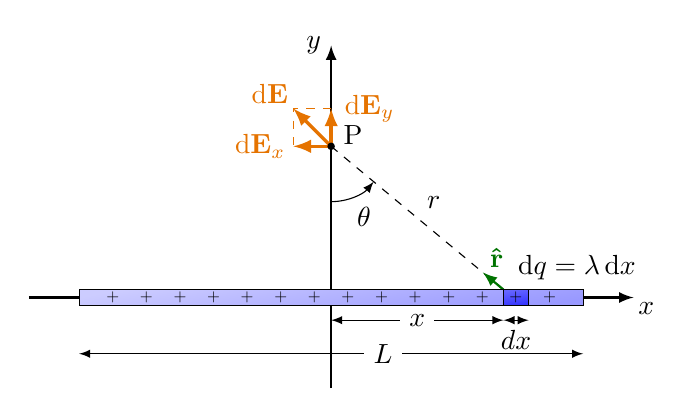
\begin{tikzpicture}[scale=0.8]
  
  \def\xmax{0.6*\L}
  \def\ymin{-0.18*\L}
  \def\ymax{0.5*\L}
  \def\x{0.342*\L}
  \def\dx{0.05*\L}
  \coordinate (O) at (0,0);
  \coordinate (P) at (0,{0.6*\ymax});
  \coordinate (X) at (\x,\W/2);
  
  % AXIS
  \draw[->,thick] (-\xmax,0) -- (\xmax,0) node[below right=-2] {$x$};
  \draw[->,thick] (0,\ymin) -- (0,\ymax) node[left] {$y$};
  
  % MEASURES
  %\draw[<->] (0,0.2*\ymax) --++ (\x,0) node[midway,above] {$x$};
  \draw[<->] (    0,0.25*\ymin) --++ (\x,0) node[measure] {$x$};
  \draw[<->] (   \x,0.25*\ymin) --++ (\dx,0) node[midway,below] {$dx$};
  \draw[<->] (-\L/2,0.62*\ymin) --++ (\L,0) node[measure,right=10] {$L$};
  
  % VECTORS
  \draw[EField,very thick] (P) --++ ( 0.0,0.6) node[right=1] {$\dd{\vb{E}_y}$};
  \draw[EField,very thick] (P) --++ (-0.6,0.0) node[left=-1] {$\dd{\vb{E}_x}$};
  \draw[EField,very thick] (P) --++ (-0.6,0.6) node[above left=-2] {$\dd{\vb{E}}$};
  \draw[EField,-,dashed,thin] (P) ++ (0,0.6) --++ (-0.6,0) --++ (0,-0.6);
  
  % POINT
  \fill (P) circle (0.06) node[above=4,right=1] {P};
  \draw[dashed] (P) -- (X) node[midway,above right] {$r$};
  \draw pic[->,"$\theta$",draw=black,angle radius=20,angle eccentricity=1.4] {angle = O--P--X};
  \draw[vector] (X) -- ($(X)!0.12!(P)$) node[right=5,above=-2] {$\vu{r}$};
  
  % ROD
  \draw[charged] (-\L/2,-\W/2) rectangle ++(\L,\W);
  \draw[darkcharged] (\x,-\W/2) rectangle ++(\dx,\W)
    node[midway,right=22,above=3] {$\dd{q}=\lambda \dd{x}$};
  \foreach \i [evaluate={\x=-\L/2+\i*\L/(\N+1);}] in {1,...,\N}{
    \node[scale=0.6] at (\x,0) {$+$};
  }
  
\end{tikzpicture}
\end{figure}


Consider a differential element of length \(d x^{\prime}\) which carries a charge \(d q=\lambda d x^{\prime}\), as shown in Figure 3.5.5. The source element is located at \(\left(x^{\prime}, 0\right)\), while the field point \(P\) is located on the \(y\)-axis at \((0, y)\). The distance from \(d x^{\prime}\) to \(P\) is \(r=\left(x^{\prime 2}+y^2\right)^{1 / 2}\). Its contribution to the potential is given by
\[
d V=\frac{1}{4 \pi \varepsilon_0} \frac{d q}{r}=\frac{1}{4 \pi \varepsilon_0} \frac{\lambda d x^{\prime}}{\left(x^{\prime 2}+y^2\right)^{1 / 2}}
\]

Taking \(V\) to be zero at infinity, the total potential due to the entire rod is
\[
\begin{aligned}
V =\frac{\lambda}{4 \pi \varepsilon_0} \underbrace{\int_{-\ell / 2}^{\ell / 2} \frac{d x^{\prime}}{\sqrt{x^{\prime 2}+y^2}}}_{\int \frac{d x^{\prime}}{\sqrt{x^{\prime 2}+y^2}}=\ln \left(x^{\prime}+\sqrt{x^{\prime 2}+y^2}\right)}=\left.\frac{\lambda}{4 \pi \varepsilon_0} \ln \left[x^{\prime}+\sqrt{x^{\prime 2}+y^2}\right]\right|_{-\ell / 2} ^{\ell / 2} =\frac{\lambda}{4 \pi \varepsilon_0} \ln \left[\frac{(\ell / 2)+\sqrt{(\ell / 2)^2+y^2}}{-(\ell / 2)+\sqrt{(\ell / 2)^2+y^2}}\right]
\end{aligned}
\]

A plot of \(V(y) / V_0\), where \(V_0=\lambda / 4 \pi \varepsilon_0\), as a function of \(y / \ell\) is shown in Figure 3.5.6

\begin{figure}[ht!]
\centering
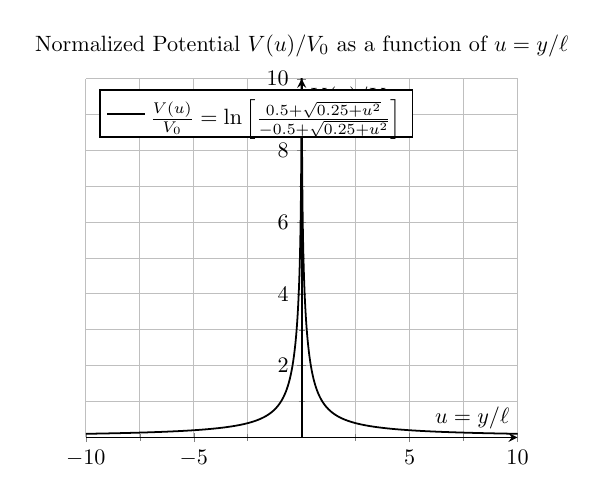
\begin{tikzpicture}[scale=0.8]
\begin{axis}[
    title={Normalized Potential $V(u) / V_0$ as a function of $u = y / \ell$},
    xlabel={$u = y / \ell$},
    ylabel={$V(u) / V_0$},
    xmin=-10, xmax=10,
    ymin=0, ymax=10,
    grid=both,
    minor tick num=1,
    legend pos=north west,
    axis lines=middle,
    smooth,
    thick,
    domain=-1:1,
    samples=4000
]
\addplot[domain=-10:10][no marks] {
    ln((0.5 + sqrt(0.25 + x^2)) / (-0.5 + sqrt(0.25 + x^2)))
};
\legend{$\frac{V(u)}{V_0} = \ln \left[\frac{0.5 + \sqrt{0.25 + u^2}}{-0.5 + \sqrt{0.25 + u^2}}\right]$}
\end{axis}
\end{tikzpicture}
\end{figure}

In the limit \(\ell \gg y\), the potential becomes
\[
\begin{aligned}
V & =\frac{\lambda}{4 \pi \varepsilon_0} \ln \left[\frac{(\ell / 2)+\ell / 2 \sqrt{1+(2 y / \ell)^2}}{-(\ell / 2)+\ell / 2 \sqrt{1+(2 y / \ell)^2}}\right]=\frac{\lambda}{4 \pi \varepsilon_0} \ln \left[\frac{1+\sqrt{1+(2 y / \ell)^2}}{-1+\sqrt{1+(2 y / \ell)^2}}\right] \\
& \approx \frac{\lambda}{4 \pi \varepsilon_0} \ln \left(\frac{2}{2 y^2 / \ell^2}\right)=\frac{\lambda}{4 \pi \varepsilon_0} \ln \left(\frac{\ell^2}{y^2}\right) \\
& =\frac{\lambda}{2 \pi \varepsilon_0} \ln \left(\frac{\ell}{y}\right)
\end{aligned}
\]

The electric field \(\vec{E}\) due to a differential element \(dq\) of the rod is given by Coulomb's law. The component of the electric field \(E_y\) at point \(P\) due to \(dq\) can be integrated over the length of the rod to find the total \(E_y\), considering symmetry and that there will be no net \(x\)-component for the entire rod:

\[
dE_y = \frac{1}{4\pi\varepsilon_0} \frac{dq}{r^2} \cos(\theta) = \frac{1}{4\pi\varepsilon_0} \frac{\lambda dx'}{y^2+x'^2} \frac{y}{\sqrt{y^2+x'^2}}
\]

Integrating \(dE_y\) over the length of the rod from \(-\ell/2\) to \(\ell/2\) gives the \(y\)-component of the electric field due to the entire rod.

\[\int_{-l/2}^{l/2} \frac{\lambda y}{4\pi \varepsilon_0 (y^2 + x^2)^{3/2}} \, dx=\frac{\lambda l}{2 \pi \varepsilon_0 y \sqrt{l^2 + 4y^2}}.\]

and it leads to the expression involving the inverse of the derivative of the potential \(V\) we obtained. The corresponding electric field can be obtained as
\[
E_y=-\frac{\partial V}{\partial y}=\frac{\lambda}{2 \pi \varepsilon_0 y} \frac{\ell / 2}{\sqrt{(\ell / 2)^2+y^2}}
\]
in complete the solution. 


\newpage
\section*{Question 5}
\addcontentsline{toc}{section}{Question 5}

\begin{q}
Show that \(\nabla \cdot \vec{D}(\vec{r}) = \rho(\vec{r})\), given \(\vec{D}(\vec{r}) = \int \frac{\rho(\vec{r}')}{4 \pi R^2} \hat{R} \, dv'\), where \(R = |\vec{R}| = |\vec{r} - \vec{r'}|\) and \(\vec{r} = (x,y,z)\)
\end{q}


Let us consider the vector field \(\vec{D}(\vec{r})\) defined by the integral
\[
\vec{D}(\vec{r}) = \int \frac{\rho(\vec{r}')}{4 \pi R^2} \hat{R} \, dv',
\]
where \(R = |\vec{R}| = |\vec{r} - \vec{r'}|\) and \(\vec{R} = \vec{r} - \vec{r'}\), with \(\vec{r}\) and \(\vec{r'}\) representing points in three-dimensional space, and \(\rho(\vec{r'})\) is a scalar function representing charge density at \(\vec{r'}\). Our goal is to demonstrate that \(\nabla \cdot \vec{D}(\vec{r}) = \rho(\vec{r})\).

The divergence of a vector field \(\vec{A} = (A_x, A_y, A_z)\) in Cartesian coordinates is given by
\[
\nabla \cdot \vec{A} = \frac{\partial A_x}{\partial x} + \frac{\partial A_y}{\partial y} + \frac{\partial A_z}{\partial z}.
\]
Applying this definition to \(\vec{D}(\vec{r})\), we need to compute the divergence of the integral expression defining \(\vec{D}\). Notice that the divergence operator acts on \(\vec{r}\) while the integral is over \(\vec{r'}\). Thus, we can interchange the order of divergence and integration due to the linearity of both operators and the fact that the integration variable \(\vec{r'}\) is independent of \(\vec{r}\).

\textit{Induction.}

Let \(\vec{F}(\vec{r}, \vec{r}')\) denote a vector field dependent upon two vector variables \(\vec{r}\) and \(\vec{r}'\), where \(\vec{r}\) is the point of evaluation in \(\mathbb{R}^3\) and \(\vec{r}'\) serves as the variable of integration over a domain \(V \subseteq \mathbb{R}^3\). The task is to demonstrate rigorously that under appropriate conditions,
\[
\nabla \cdot \int_V \vec{F}(\vec{r}, \vec{r}') \, dV' = \int_V \nabla \cdot \vec{F}(\vec{r}, \vec{r}') \, dV',
\]
it is implicitly understood that \(\vec{F}\) is sufficiently smooth, and that the domain of integration and the vector field \(\vec{F}\) itself satisfy conditions permitting the interchange of integration and differentiation.

Proceed by acknowledging the definition of the divergence operator in Cartesian coordinates for a vector field \(\vec{G}(\vec{r}) = (G_x(\vec{r}), G_y(\vec{r}), G_z(\vec{r}))\), which is
\[
\nabla \cdot \vec{G} = \frac{\partial G_x}{\partial x} + \frac{\partial G_y}{\partial y} + \frac{\partial G_z}{\partial z}.
\]

The application of this operator to the integral expression yields
\[
\nabla \cdot \int_V \vec{F}(\vec{r}, \vec{r}') \, dV' = \frac{\partial}{\partial x} \int_V F_x(\vec{r}, \vec{r}') \, dV' + \frac{\partial}{\partial y} \int_V F_y(\vec{r}, \vec{r}') \, dV' + \frac{\partial}{\partial z} \int_V F_z(\vec{r}, \vec{r}') \, dV',
\]
assuming that \(F_x\), \(F_y\), and \(F_z\) are the components of \(\vec{F}\).

To interchange differentiation and integration, \underline{invoke Leibniz’s rule} for differentiation under the integral sign, which stipulates that if \(\vec{F}\) and its partial derivatives with respect to \(\vec{r}\) are continuous over the domain of integration, then differentiation with respect to \(\vec{r}\) can indeed be interchanged with the integration with respect to \(\vec{r}'\).
\[
\frac{\partial}{\partial x_i} \int_V F_j(\vec{r}, \vec{r}') \, dV' = \int_V \frac{\partial F_j(\vec{r}, \vec{r}')}{\partial x_i} \, dV',
\]
for \(i = 1, 2, 3\) corresponding to the Cartesian coordinates \(x\), \(y\), and \(z\), and for each component \(j\) of \(\vec{F}\).

Thus, applying the above principle yields
\[
\nabla \cdot \int_V \vec{F}(\vec{r}, \vec{r}') \, dV' = \int_V \left(\frac{\partial F_x}{\partial x} + \frac{\partial F_y}{\partial y} + \frac{\partial F_z}{\partial z}\right) \, dV' = \int_V \nabla \cdot \vec{F}(\vec{r}, \vec{r}') \, dV',
\]
where the final expression utilizes the definition of divergence in terms of the components of \(\vec{F}\).

Therefore,
\[
\nabla \cdot \vec{D}(\vec{r}) = \nabla \cdot \int \frac{\rho(\vec{r}')}{4 \pi R^2} \hat{R} \, dv' = \int \nabla \cdot \left(\frac{\rho(\vec{r}')}{4 \pi R^2} \hat{R}\right) \, dv'.
\]

\hline

To proceed, we recognize that \(\nabla \cdot (\hat{R}/R^2) = 4\pi \delta(\vec{R})\) in three dimensions, where \(\delta(\vec{R})\) is the three-dimensional Dirac delta function centered at \(\vec{R} = 0\) or equivalently at \(\vec{r} = \vec{r'}\). This is a consequence of the divergence theorem and the properties of the Green's function for the Laplacian in three dimensions.


For a fixed \(x_0\), define \(G_{x_0}=\left|x-x_0\right|^{-1}\). Then \(\nabla^2 G_{x_0}=0\) for \(x \neq x_0\). If \(\varphi\) is a compactly supported \(C^{\infty}\) function on \(\mathbb{R}^3\), then
\[
\nabla \cdot\left(G_{x_0} \nabla \varphi-\varphi \nabla G_{x_0}\right)=G_{x_0} \nabla^2 \varphi-\varphi \nabla^2 G_{x_0}=G_{x_0} \nabla^2 \varphi, \quad x \neq x_0 .
\]

Integrate and apply the divergence theorem, keeping in mind that \(\varphi\) vanishes outside a large sphere:
\[
\begin{aligned}
\int_{\mathbb{R}^3} G_{x_0} \nabla^2 \varphi d V & =\lim _{\epsilon \downarrow 0} \int_{\left|x-x_0\right| \geq \epsilon} G_{x_0} \nabla^2 \varphi d V \\
& =-\lim _{\epsilon \downarrow 0} \int_{\left|x-x_0\right| \geq \epsilon} \nabla \cdot\left(\varphi \nabla G_{x_0}-G_{x_0} \nabla \varphi\right) d V \\
& =-\lim _{\epsilon \downarrow 0} \int_{\left|x-x_0\right|=\epsilon}\left(\varphi \frac{\partial G_{x_0}}{\partial n}-G_{x_0} \frac{\partial \varphi}{\partial n}\right) d S \\
& =-\lim _{\epsilon \downharpoonright 0} \int_{\left|x-x_0\right|=\epsilon} \varphi \frac{\partial G_{x_0}}{\partial n} d S
\end{aligned}
\]

Like

\[
D^\alpha T: \varphi \mapsto(-1)^{|\alpha|} T\left[D^\alpha \varphi\right]
\]
for higher derivatives.
From that we obtain \(\left(\nabla^2 T\right)[\varphi]=T\left[\nabla^2 \varphi\right]\), and for the locally integrable function \(f(x)=\left\|x-x_0\right\|^{-1}\) we therefore have
\[
\left(\nabla^2 T_f\right)[\varphi]=T\left[\nabla^2 \varphi\right]=\int_{\mathbb{R}^3} f(x) \cdot \nabla^2 \varphi(x) d x_1 d x_2 d x_3 .
\]

Now choose \(R>0\) so large that \(\operatorname{supp} \varphi \subset B_R\left(x_0\right)\), and choose \(0<\varepsilon<R\). Then
\[
\int_{\mathbb{R}^3} f(x) \cdot \nabla^2 \varphi(x) d x_1 d x_2 d x_3=\lim _{\varepsilon \searrow 0} \int_{\varepsilon<\left\|x-x_0\right\|<R} f(x) \cdot \nabla^2 \varphi(x) d x_1 d x_2 d x_3
\]
since \(f\) is locally integrable and \(\nabla^2 \varphi\) is continuous.
Away from \(x_0, f\) is smooth, and a slightly tedious computation shows that \(\nabla^2 f \equiv 0\) on \(\mathbb{R}^3 \backslash\left\{x_0\right\}\), so
\[
\int_{\mathbb{R}^3} f(x) \cdot \nabla^2 \varphi(x) d x_1 d x_2 d x_3=\lim _{\varepsilon \lambda_0} \int_{\varepsilon<\left\|x-x_0\right\|<R} f(x) \cdot \nabla^2 \varphi(x)-\varphi(x) \cdot \nabla^2 f(x) d x_1 d x_2 d x_3
\]



The normal derivative is in the inward direction on \(\left|x-x_0\right|=\epsilon\) because the outward normal on \(\epsilon \leq\left|x-x_0\right| \leq R\) is where this started. \(G_{x_0}(x)=1 / r\) for \(\left|x-x_0\right|=r\). So you end up with a normal derivative of \(G_{x_0}\) equal to \(1 / \epsilon^2\) on \(\left|x-x_0\right|=\epsilon\). Therefore, you pick up a factor equal to the area of the unit sphere:
\[
\int_{\mathbb{R}^3} G_{x_0} \nabla^2 \varphi d V=-\lim _{\epsilon \downarrow 0} \frac{1}{\epsilon^2} \int_{\left|x-x_0\right|=\epsilon} \varphi(x) d S=-4 \pi \varphi\left(x_0\right) .
\]


and to that integral we can apply Green's formula to obtain
\[
\begin{aligned}
& \int_{\mathbb{R}^3} f(x) \cdot \nabla^2 \varphi(x) d x_1 d x_2 d x_3= \lim _{\varepsilon \searrow_0}\left(\int_{\left\|x-x_0\right\|=R} f(x) \frac{\partial \varphi}{\partial \nu}(x)-\varphi(x) \frac{\partial f}{\partial \nu}(x) d S\right. \\
&\left.\quad+\int_{\left\|x-x_0\right\|=\varepsilon} f(x) \frac{\partial \varphi}{\partial \nu}(x)-\varphi(x) \frac{\partial f}{\partial \nu}(x) d S\right) \\
&=\lim _{\varepsilon\rangle_0} \int_{\left\|x-x_0\right\|=\varepsilon} f(x) \frac{\partial \varphi}{\partial \nu}(x)-\varphi(x) \frac{\partial f}{\partial \nu}(x) d S
\end{aligned}
\]
where \(d S\) denotes the surface measure of the sphere, \(\frac{\partial}{\partial \nu}\) the directional derivative in direction of the outer normal, and the first integral on the right hand side vanishes since \(\varphi\) vanishes in a neighbourhood of the outer sphere. The outer normal on the sphere \(\left\|x-x_0\right\|=\varepsilon\) is \(-\frac{x-x_0}{\left\|x-x_0\right\|}\),
so we are left with
\[
\frac{1}{\varepsilon} \int_{\left\|x-x_0\right\|=\varepsilon} f(x)\left\langle\nabla \varphi(x), x-x_0\right\rangle-\varphi(x)\left\langle\nabla f, x-x_0\right\rangle d S .
\]

An easy estimate shows
\[
\frac{1}{\varepsilon} \int_{\left\|x-x_0\right\|=\varepsilon} f(x)\left\langle\nabla \varphi(x), x-x_0\right\rangle d S \leqslant \frac{1}{\varepsilon^2} \int_{\left\|x-x_0\right\|=\varepsilon}\|\nabla \varphi\| \cdot \varepsilon d S \leqslant C \frac{4 \pi \varepsilon^2}{\varepsilon} \xrightarrow{\varepsilon \searrow 0} 0 .
\]

For the other part of the integral, computing \(\frac{\partial f}{\partial \nu}\) gives
\[
\int_{\left\|x-x_0\right\|=\varepsilon} \varphi(x) \cdot \frac{1}{\varepsilon^2} d S,
\]

and since \(\varphi\) is continuous at \(x_0\) we have
\[
\lim _{\varepsilon \searrow 0} \int_{\left\|x-x_0\right\|=\varepsilon} \varphi(x) \cdot \frac{1}{\varepsilon^2} d S=4 \pi \varphi\left(x_0\right) .
\]

Collecting everything without mucking up the signs, we get
\[
\left(\nabla^2 f\right)[\varphi]=\int_{\mathbb{R}^3} f(x) \cdot \nabla^2 \varphi(x) d x_1 d x_2 d x_3=-4 \pi \varphi\left(x_0\right)=-4 \pi \delta_{x_0}[\varphi] .
\]

That holds for all test functions \(\varphi\), hence \(\nabla^2 f=-4 \pi \delta_{x_0}\).


\textit{Another way.}

We have\[\frac{1}{r}=\frac{1}{\sqrt{x^2+y^2+z^2}} \in \mathbb{L}_{l o c}^1\left(\mathbb{R}^3\right)\]Since\[-\nabla \frac{1}{r}=\frac{\hat{r}}{r^2}\]We have\[\vec{\nabla} \cdot \frac{\hat{r}}{r^2}=-\nabla^2 \frac{1}{r}\]The classical derivative of this function vanishes everywhere except at \(r=0\) where it does not exist. In other words, \(\frac{1}{r}\) is Harmonic \({ }^{[1]}\) on \(\mathbb{R}^3 / \mathbf{0}\).So we extend(something that is not in general possible for an arbitrary function but always possible for a everywhere locally integrable \({ }^{[2]}\) function to a distribution, in this case, on the whole of \(\mathbb{R}^3\) ) \(\frac{1}{r}\) as a distribution (aka a continuous linear functional) to the whole \(\mathbb{R}\) on the space of test functions(in this case that could be the space of smooth functions with compact support or the Schwartz space \({ }^{[3]}\) ). This allows us to differentiate it as a distribution which are infinitely differentiable(in the distributional sense).\[\left\langle\nabla^2 \frac{1}{r}, \varphi>:=<\frac{1}{r}, \nabla^2 \varphi>\right.\]where \(\varphi \in C_c^{\infty}\left(\mathbb{R}^3\right) \operatorname{or} S\left(\mathbb{R}^3\right)\) \[<\frac{1}{r}, \nabla^2 \varphi>=\lim _{\epsilon \rightarrow 0^{+}} \iiint_{r \geq \epsilon} \frac{\nabla^2 \varphi}{r} d V\]where we are integrating over the spherical shell(layer) \(\epsilon \leq r \leq a\) and where a is so large that \(\varphi\) vanishes outside \(\boldsymbol{r}=\boldsymbol{a}\). (in other words we let \(\boldsymbol{a} \rightarrow \infty\) and exploit the compact support or the rapidly decaying property of our functions).Then by using Green's second identity \({ }^{[4]}\) what we are left with is\[\iiint_{r \geq \epsilon} \frac{\nabla^2 \varphi}{r} d V=\iiint_{r \geq \epsilon} \varphi \nabla^2 \frac{1}{r} d V-\iint_{r=\epsilon} \frac{\partial \varphi}{\partial r} \frac{1}{r} d S+\iint_{r=\epsilon} \varphi \frac{\partial}{\partial r} \frac{1}{r} d S\]where \(d S\) is the element of area(aka area measure) on the sphere of radius \(\epsilon\).Since \(\frac{1}{r}\) is harmonic outside the ball \(r=\epsilon\) Thus\[\iiint_{r \geq \epsilon} \varphi \nabla^2 \frac{1}{r} d V=0\]Next\[\iint_{r=\epsilon} \frac{\partial \varphi}{\partial r} \frac{1}{r} d S=\frac{1}{\epsilon} \iint_{r=\epsilon} \frac{\partial \varphi}{\partial r} d S=O(\epsilon)\]where the last equality holds because of the compact support(or rapidly decaying in case of Schwartz space) property of our functions.Finally\[\iint_{r=\epsilon} \varphi \frac{\partial}{\partial r} \frac{1}{r} d S=-\frac{1}{\epsilon^2} \iint_{r=\epsilon} \varphi d S=-4 \pi \frac{1}{4 \pi \epsilon^2} \iint_{r=\epsilon} \varphi d S\] Here\[\frac{1}{4 \pi \epsilon^2} \iint_{T=\epsilon} \varphi d S\]is the mean value \({ }^{[5]}\) of \(\varphi\) over the sphere \(r=\epsilon\) which approaches \(\varphi(\overrightarrow{0})\) as \(\epsilon \rightarrow 0^{+}\).Hence\[\begin{aligned}& <\nabla^2 \frac{1}{r}, \varphi>=\lim _{\epsilon \rightarrow 0^{+}} \iiint_{r \geq \epsilon} \frac{\nabla^2 \varphi}{r} d V=-4 \pi \varphi(\overrightarrow{0})=\langle-4 \pi \delta, \varphi\rangle \\& \Longrightarrow \nabla^2 \frac{1}{r}=-4 \pi \delta\end{aligned}\]Thus we get the desired result\[\vec{\nabla} \cdot \frac{\hat{r}}{r^2}=4 \pi \delta\]

\hline

Therefore, by applying this identity and noting that \(\rho(\vec{r}')\) is a scalar function that can be taken out of the divergence operator, the integral becomes
\[
\int \nabla \cdot \left(\frac{\rho(\vec{r}')}{4 \pi R^2} \hat{R}\right) \, dv' = \int \rho(\vec{r}') \delta(\vec{r} - \vec{r'}) \, dv'.
\]

Let \(\vec{r}\) and \(\vec{r'}\) denote points in \(\mathbb{R}^3\), with \(\vec{r}\) fixed and \(\vec{r'}\) variable, and let \(\rho: \mathbb{R}^3 \rightarrow \mathbb{R}\) be a scalar field representing a physical quantity such as charge density. The Dirac delta function, \(\delta(\vec{r} - \vec{r'})\), is a distribution with the property that for any sufficiently smooth function \(f: \mathbb{R}^3 \rightarrow \mathbb{R}\),
\[
\int f(\vec{r'}) \delta(\vec{r} - \vec{r'}) \, dv' = f(\vec{r}),
\]
where the integration is taken over the entire space \(\mathbb{R}^3\).

So, basically, from the definition of the Dirac delta function, the integral on the right-hand side will equal 1, thus the integration over the volume with the delta function effectively evaluates \(\rho\) at \(\vec{r} = \vec{r'}\), yielding
\[
\int \rho(\vec{r}') \delta(\vec{r} - \vec{r'}) \, dv' = \rho(\vec{r}).
\]
Hence, we have shown that
\[
\boxed{\nabla \cdot \vec{D}(\vec{r}) = \rho(\vec{r})}.
\]


\newpage
\section*{Question 6}
\addcontentsline{toc}{section}{Question 6}
\begin{q}
Determine the electric field intensity \(\vec{E}\) on the \(z\) axis due to a square loop of uniform line charge density \(\rho_L\) with side \(a\) located in the \(x-y\) plane with two different methods and compare them.
\end{q}

\textit{From center.}

We see that the electric field a distance \(r\) from a line of uniformly distributed charge of length \(2 L\) is

The simplest method is to chop the line into symmetrically placed pairs (at \(\pm x\) ), quote the result of Ex. 2.1 (with \(d / 2 \rightarrow x, q \rightarrow \lambda d x\) ), and integrate \((x: 0 \rightarrow L\) ). But here's a more general approach: (Ordinarily I’ll put a prime on the source coordinates, but where no confusion can arise I’ll remove the prime to simplify the notation.)
\[
\begin{aligned}
& \mathbf{r}=z \hat{\mathbf{z}}, \quad \mathbf{r}^{\prime}=x \hat{\mathbf{x}}, \quad d l^{\prime}=d x ; \\
& r=\mathbf{r}-\mathbf{r}^{\prime}=z \hat{\mathbf{z}}-x \hat{\mathbf{x}}, \quad r=\sqrt{z^2+x^2}, \quad \hat{\imath}=\frac{r}{r}=\frac{z \hat{\mathbf{z}}-x \hat{\mathbf{x}}}{\sqrt{z^2+x^2}} \text {. } \\
& \mathbf{E}=\frac{1}{4 \pi \epsilon_0} \int_{-L}^L \frac{\lambda}{z^2+x^2} \frac{z \hat{\mathbf{z}}-x \hat{\mathbf{x}}}{\sqrt{z^2+x^2}} d x \\
& =\frac{\lambda}{4 \pi \epsilon_0}\left[z \hat{\mathbf{z}} \int_{-L}^L \frac{1}{\left(z^2+x^2\right)^{3 / 2}} d x-\hat{\mathbf{x}} \int_{-L}^L \frac{x}{\left(z^2+x^2\right)^{3 / 2}} d x\right] \\
& =\frac{\lambda}{4 \pi \epsilon_0}\left[\left.z \hat{\mathbf{z}}\left(\frac{x}{z^2 \sqrt{z^2+x^2}}\right)\right|_{-L} ^L-\left.\hat{\mathbf{x}}\left(-\frac{1}{\sqrt{z^2+x^2}}\right)\right|_{-L} ^L\right] \\
& =\frac{1}{4 \pi \epsilon_0} \frac{2 \lambda L}{z \sqrt{z^2+L^2}} \hat{\mathbf{z}} . \\
&
\end{aligned}
\]


\[
\vec{E}(\vec{r})=\frac{1}{4 \pi \epsilon_0} \frac{2 \lambda L}{r \sqrt{r^2+L^2}} \hat{r}
\]
where \(\vec{r}\) points directly away from the center of the line and perpindicular to it. So, to find the field a distance \(z\) from the center of the square loop shown in the figure we need to just sum up four such electric fields.

The distance from the point \(P\) to any of the four sides of the square will be \(r=\sqrt{z^2+\left(\frac{a}{2}\right)^2}\). Each contribution to the electric field will have a component in the \(z\) direction as well as a component parallel to the plane of the square loop. However, these parallel components sum to zero because of the symmetry of the loop. Therefore, we just need to add up the \(z\) components to find the total \(\vec{E}\) :
\[
\begin{aligned}
\vec{E}(z) & =4\left[\frac{1}{4 \pi \epsilon_0} \frac{2 \lambda L}{r \sqrt{r^2+L^2}}\right] \sin \theta_r \hat{z} \\
& =\frac{1}{\pi \epsilon_0} \frac{2 \lambda \frac{a}{2}}{r \sqrt{r^2+\left(\frac{a}{2}\right)^2}} \frac{z}{r} \hat{z} \\
& =\boxed{\frac{1}{\pi \epsilon_0} \frac{\lambda a z}{\left(z^2+\frac{a^2}{4}\right) \sqrt{z^2+\frac{a^2}{2}}} \hat{z}} .
\end{aligned}
\]
\textit{Above any point.}

The expression of the electric field from the Coulomb law is:
\[
\vec{E}(x, y, z)=\frac{1}{4 \pi \varepsilon_0} \int_{u=-a}^a \int_{v=-b}^b \frac{\sigma}{\left((x-u)^2+(y-v)^2+z^2\right)^{3 / 2}}\left((x-u) \hat{e}_x+(y-v) \hat{e}_y+z \hat{e}_z\right) \mathrm{d} u \mathrm{~d} v
\]

We start with the component \(E_x\) :
\[
E_x(x, y, z)=\frac{\sigma}{4 \pi \varepsilon_0} \int_{u=-a}^a \int_{v=-b}^b \frac{(x-u) \mathrm{d} u \mathrm{~d} v}{\left((x-u)^2+(y-v)^2+z^2\right)^{3 / 2}}
\]

The integration over \(x\) is straightforward:
\[
\begin{aligned}
E_x(x, y, z) & =\frac{\sigma}{4 \pi \varepsilon_0} \int_{v=-b}^b\left[\frac{-1}{\left((x-u)^2+(y-v)^2+z^2\right)^{1 / 2}}\right]_{u=-a}^a \mathrm{~d} v \\
& =\frac{\sigma}{4 \pi \varepsilon_0} \int_{v=-b}^b\left[\frac{1}{\left((x+a)^2+(y-v)^2+z^2\right)^{1 / 2}}-\frac{1}{\left((x-a)^2+(y-v)^2+z^2\right)^{1 / 2}}\right] \mathrm{d} v
\end{aligned}
\]

The derivative of the function \(\operatorname{argsh}(x)\) is \(\frac{1}{\sqrt{x^2+1}}\), which tells us how to perform the integration. We introduce \(c_{ \pm}=\sqrt{(x \pm a)^2+z^2}\) and \(p=\frac{y-v}{c_{+}}, q=\frac{y-v}{c_{-}}\)and we obtain the result for \(E_x\). Note that there is no minus sign because the invert the limits and \(c_{+} \mathrm{d} p=-\mathrm{d} u, c_{-} \mathrm{d} q=-\mathrm{d} v\).
\[
\begin{aligned}
& E_x(x, y, z)=\frac{\sigma}{4 \pi \varepsilon_0}\left[\int_{p=\frac{y-b}{c_{+}}}^{p=\frac{y+b}{c_{+}}} \frac{c_{+} \mathrm{d} p}{c_{+} \sqrt{p^2+1}}-\int_{q=\frac{y-b}{c_{-}}}^{q=\frac{y+b}{c_{-}}} \frac{c_{-} \mathrm{d} q}{c_{-} \sqrt{q^2+1}}\right] \\
&=\frac{\sigma}{4 \pi \varepsilon_0}\left[\operatorname{argsh}\left(\frac{y+b}{c_{+}}\right)-\operatorname{argsh}\left(\frac{y-b}{c_{+}}\right)-\operatorname{argsh}\left(\frac{y+b}{c_{-}}\right)+\operatorname{argsh}\left(\frac{y-b}{c_{-}}\right)\right] \\
& E_x(x, y, z)=\frac{\sigma}{4 \pi \varepsilon_0} {\left[\operatorname{argsh}\left(\frac{y+b}{\sqrt{(x+a)^2+z^2}}\right)-\operatorname{argsh}\left(\frac{y-b}{\sqrt{(x+a)^2+z^2}}\right)\right.} \\
&\left.-\operatorname{argsh}\left(\frac{y+b}{\sqrt{(x-a)^2+z^2}}\right)+\operatorname{argsh}\left(\frac{y-b}{\sqrt{(x-a)^2+z^2}}\right)\right]
\end{aligned}
\]
Similarly, we get \(E_y\) :
\[
\begin{aligned}
E_y(x, y, z)=\frac{\sigma}{4 \pi \varepsilon_0}[ & \operatorname{argsh}\left(\frac{x+a}{\sqrt{(y+b)^2+z^2}}\right)-\operatorname{argsh}\left(\frac{x-a}{\sqrt{(y+b)^2+z^2}}\right) \\
& \left.-\operatorname{argsh}\left(\frac{x+a}{\sqrt{(y-b)^2+z^2}}\right)+\operatorname{argsh}\left(\frac{x-a}{\sqrt{(y-b)^2+z^2}}\right)\right]
\end{aligned}
\]

The calculation of \(E_z\) is different:
\[
E_z(x, y, z)=\frac{\sigma}{4 \pi \varepsilon_0} \int_{u=-a}^a \int_{v=-b}^b \frac{z \mathrm{~d} u \mathrm{~d} v}{\left((x-u)^2+(y-v)^2+z^2\right)^{3 / 2}}
\]

We start with \(X=x-u\) and \(Y=y-v\). Note again that there is no minus sign because the invert the limits and \(\mathrm{d} X=-\mathrm{d} u, \mathrm{~d} Y=-\mathrm{d} v\).
\[
E_z(x, y, z)=\frac{\sigma}{4 \pi \varepsilon_0} \int_{X=x-a}^{x+a} \int_{Y=y-b}^{y+b} \frac{z \mathrm{~d} X \mathrm{~d} Y}{\left(X^2+Y^2+z^2\right)^{3 / 2}}
\]

Now we introduce \(\theta\) such as \(Y=\sqrt{X^2+z^2} \tan \theta\). We have \(\mathrm{d} Y=\sqrt{X^2+z^2} \frac{\mathrm{d} \theta}{\cos ^2 \theta}\) and \(1+\tan ^2 \theta=\frac{1}{\cos ^2 \theta}\). We get:
\[
\begin{aligned}
E_z(x, y, z) & =\frac{\sigma z}{4 \pi \varepsilon_0} \int_{X=x-a}^{x+a} \int_{\theta=\arctan \left(y-b / \sqrt{X^2+z^2}\right)}^{\arctan \left(y+b / \sqrt{X^2+z^2}\right)} \frac{\sqrt{X^2+z^2} \mathrm{~d} \theta}{\cos ^2 \theta\left(\left(X^2+z^2\right)\left(1+\tan ^2 \theta\right)\right)^{3 / 2}} \mathrm{~d} X \\
& =\frac{\sigma z}{4 \pi \varepsilon_0} \int_{X=x-a}^{x+a} \frac{\mathrm{d} X}{X^2+z^2} \int_{\theta=\arctan \left(y-b / \sqrt{X^2+z^2}\right)}^{\arctan \left(y+b / \sqrt{X^2+z^2}\right)} \cos \theta \mathrm{d} \theta \\
& =\frac{\sigma z}{4 \pi \varepsilon_0} \int_{X=x-a}^{x+a} \frac{\mathrm{d} X}{X^2+z^2}\left[\sin \left(\arctan \left(\frac{y+b}{\sqrt{X^2+z^2}}\right)\right)-\sin \left(\arctan \left(\frac{y-b}{\sqrt{X^2+z^2}}\right)\right)\right]
\end{aligned}
\]

Since \(\arctan \psi=\arcsin \left(\frac{\psi}{\sqrt{1+\psi^2}}\right)\), we obtain:
\[
\begin{aligned}
E_z(x, y, z) & =\frac{\sigma z}{4 \pi \varepsilon_0} \int_{X=x-a}^{x+a} \frac{\mathrm{d} X}{X^2+z^2}\left[\frac{\frac{y+b}{\sqrt{X^2+z^2}}}{\sqrt{1+\frac{(y+b)^2}{X^2+z^2}}}-\frac{\frac{y-b}{\sqrt{X^2+z^2}}}{\sqrt{1+\frac{(y-b)^2}{X^2+z^2}}}\right] \\
& =\frac{\sigma z}{4 \pi \varepsilon_0} \int_{X=x-a}^{x+a} \frac{\mathrm{d} X}{X^2+z^2}\left[\frac{y+b}{\sqrt{(y+b)^2+X^2+z^2}}-\frac{y-b}{\sqrt{(y-b)^2+X^2+z^2}}\right]
\end{aligned}
\]

We introduce \(\theta\) and \(\varphi\) such as \(X=\sqrt{(y+b)^2+z^2} \tan \theta\), and thus \(\mathrm{d} X=\sqrt{(y+b)^2+z^2} \frac{\mathrm{d} \theta}{\cos ^2 \theta}\) in the first part and \(X=\sqrt{(y-b)^2+z^2} \tan \varphi\), and thus \(\mathrm{d} X=\sqrt{(y-b)^2+z^2} \frac{\mathrm{d} \varphi}{\cos ^2 \varphi}\) in the second part. We obtain:
\[
\begin{aligned}
& E_z(x, y, z)=\\
&\frac{\sigma z}{4 \pi \varepsilon_0}\left[\int_{\arctan \left(x-a / \sqrt{(y+b)^2+z^2}\right)}^{\arctan \left(x+a / \sqrt{(y+b)^2+z^2}\right)} \frac{(y+b) \sqrt{(y+b)^2+z^2} \mathrm{~d} \theta}{\left(\left((y+b)^2+z^2\right) \tan ^2 \theta+z^2\right) \cos ^2 \theta \sqrt{\left((y+b)^2+z^2\right)\left(1+\tan ^2 \theta\right)}}\right. \\
&\left.-\int_{\arctan \left(x-a / \sqrt{(y-b)^2+z^2}\right)}^{\arctan \left(x+a / \sqrt{(y-b)^2+z^2}\right)} \frac{(y-b) \sqrt{(y-b)^2+z^2} \mathrm{~d} \varphi}{\left(\left((y-b)^2+z^2\right) \tan ^2 \varphi+z^2\right) \cos ^2 \varphi \sqrt{\left((y-b)^2+z^2\right)\left(1+\tan ^2 \varphi\right)}}\right]
\end{aligned}
\]
After cleaning up everything, we have:
\[
\begin{aligned}
E_z(x, y, z)=\frac{\sigma z}{4 \pi \varepsilon_0}[ & \int_{\arctan \left(x-a / \sqrt{(y+b)^2+z^2}\right)}^{\arctan \left(x+a / \sqrt{(y+b)^2+z^2}\right)} \frac{(y+b) \mathrm{d} \theta}{\left(\left((y+b)^2+z^2\right) \tan ^2 \theta+z^2\right) \cos \theta} \\
& \left.-\int_{\arctan \left(x-a / \sqrt{(y-b)^2+z^2}\right)}^{\arctan \left(x+a / \sqrt{(y-b)^2+z^2}\right)} \frac{(y-b) \mathrm{d} \varphi}{\left(\left((y-b)^2+z^2\right) \tan ^2 \varphi+z^2\right) \cos \varphi}\right]
\end{aligned}
\]

Since \(\left((y+b)^2+z^2\right) \tan ^2 \theta+z^2=\frac{(y+b)^2 \sin ^2 \theta+z^2}{\cos ^2 \theta}\), we can rewrite it as:
\[
\begin{aligned}
E_z(x, y, z)=\frac{\sigma z}{4 \pi \varepsilon_0}[ & \int_{\arctan \left(x-a / \sqrt{(y+b)^2+z^2}\right)}^{\arctan \left(x+a / \sqrt{(y+b)^2+z^2}\right)} \frac{(y+b) \cos \theta \mathrm{d} \theta}{(y+b)^2 \sin ^2 \theta+z^2} \\
& \left.-\int_{\arctan \left(x-a / \sqrt{(y-b)^2+z^2}\right)}^{\arctan \left(x+a / \sqrt{(y-b)^2+z^2}\right)} \frac{(y-b) \cos \varphi \mathrm{d} \varphi}{(y-b)^2 \sin ^2 \varphi+z^2}\right]
\end{aligned}
\]

We introduce:
\[
\begin{aligned}
& U=\frac{(y+b) \sin \theta}{z}, \mathrm{~d} U=\frac{y+b}{z} \cos \theta \mathrm{d} \theta \\
& V=\frac{(y-b) \sin \varphi}{z}, \mathrm{~d} V=\frac{y-b}{z} \cos \varphi \mathrm{d} \varphi
\end{aligned}
\]

The boundaries of the integrals are then defined by:
\[
\begin{aligned}
f(x \pm a, y \pm b) & =\frac{y \pm b}{z} \sin \left(\arctan \left(\frac{x \pm a}{\sqrt{(y \pm b)^2+z^2}}\right)\right) \\
& =\frac{y \pm b}{z} \frac{x \pm a}{\sqrt{(y \pm b)^2+z^2+(x \pm a)^2}}
\end{aligned}
\]

When we insert this in the expression of \(E_z\), we obtain:
\[
\begin{aligned}
E_z(x, y, z) & =\frac{\sigma z}{4 \pi \varepsilon_0}\left[\int_{U=f(x-a, y+b)}^{f(x+a, y+b)}(y+b) \frac{z}{y+b} \frac{1}{z^2} \frac{\mathrm{d} U}{U^2+1}-\int_{V=f(x-a, y-b)}^{f(x+a, y-b)}(y-b) \frac{z}{y-b} \frac{1}{z^2} \frac{\mathrm{d} V}{V^2+1}\right] \\
& =\frac{\sigma}{4 \pi \varepsilon_0}\left[[\arctan U]_{U=f(x-a, y+b)}^{f(x+a, y+b)}-[\arctan V]_{V=f(x-a, y-b)}^{f(x+a, y-b)}\right] \\
& =\frac{\sigma}{4 \pi \varepsilon_0}\left[\arctan \left(\frac{y+b}{z} \frac{x+a}{\sqrt{(y+b)^2+z^2+(x+a)^2}}\right)-\arctan \left(\frac{y+b}{z} \frac{x-a}{\sqrt{(y+b)^2+z^2+(x-a)^2}}\right)\right. \\
& \left.-\arctan \left(\frac{y-b}{z} \frac{x-a}{\sqrt{(y-b)^2+z^2+(x+a)^2}}\right)+\arctan \left(\frac{y-b}{z} \frac{x-a}{\sqrt{(y-b)^2+z^2+(x-a)^2}}\right)\right]
\end{aligned}
\]
To summarize:
\[
\begin{aligned}
& E_x(x, y, z)=\frac{\sigma}{4 \pi \varepsilon_0}[ \operatorname{argsh}\left(\frac{y+b}{\sqrt{(x+a)^2+z^2}}\right)-\operatorname{argsh}\left(\frac{y-b}{\sqrt{(x+a)^2+z^2}}\right) \\
&\left.-\operatorname{argsh}\left(\frac{y+b}{\sqrt{(x-a)^2+z^2}}\right)+\operatorname{argsh}\left(\frac{y-b}{\sqrt{(x-a)^2+z^2}}\right)\right] \\
& E_y(x, y, z)=\frac{\sigma}{4 \pi \varepsilon_0}[ \operatorname{argsh}\left(\frac{x+a}{\sqrt{(y+b)^2+z^2}}\right)-\operatorname{argsh}\left(\frac{x-a}{\sqrt{(y+b)^2+z^2}}\right) \\
&\left.-\operatorname{argsh}\left(\frac{x+a}{\sqrt{(y-b)^2+z^2}}\right)+\operatorname{argsh}\left(\frac{x-a}{\sqrt{(y-b)^2+z^2}}\right)\right] \\
& E_z(x, y, z)=\frac{\sigma}{4 \pi \varepsilon_0}[ \arctan \left(\frac{y+b}{z} \frac{x+a}{\left.\sqrt{(y+b)^2+z^2+(x+a)^2}\right)-\arctan \left(\frac{y+b}{z} \frac{x-a}{\sqrt{(y+b)^2+z^2+(x-a)^2}}\right)}\right) \\
&\left.-\arctan \left(\frac{y-b}{z} \frac{x-a}{\sqrt{(y-b)^2+z^2+(x+a)^2}}\right)+\arctan \left(\frac{y-b}{z} \frac{x}{\sqrt{(y-b)^2+z^2+(x-a)^2}}\right)\right]
\end{aligned}
\]

\textbf{Comparison of Methods.}

Second one is hard.


\newpage
\section*{Question 7}
\addcontentsline{toc}{section}{Question 7}
\begin{q}
A very long cylindrical object consists of an inner cylinder of radius \(a\), which has a uniform charge density \(\rho\), and a concentric thin cylinder, of radius \(b\), which has an equal but opposite total charge, uniformly distributed on the surface.
(a) (7 points) Calculate the electric field everywhere.
(b) (6 points) Calculate the electric potential everywhere, taking \(V=0\) on the outer cylinder.
(c) (7 points) Calculate the electrostatic energy per unit length of the object.
\end{q}


(a) This problem has enough symmetry to allow a solution by Gauss's law. In particular, symmetry considerations imply that the electric field will point radially outward, and will have a magnitude that depends only on the distance from the axis. Following Griffiths, we use \(s\) for the distance from the \(z\)-axis, and \(\hat{s}\) for a unit vector pointing radially outward from the axis, and of course we choose the \(z\)-axis to be the axis of the cylindrical object. Then
\[
\vec{E}=E(s) \hat{s} .
\]

To evaluate \(E(s)\), we apply Gauss's law to a Gaussian cylinder of length \(\ell\), concentric with the \(z\)-axis. Then
\[
\oint \vec{E} \cdot \mathrm{d} \vec{a}=\frac{Q_{\mathrm{enc}}}{\epsilon_0}=2 \pi s \ell E(s) .
\]

For \(s<a\), the Gaussian cylinder is filled with charge density \(\rho\), so
\[
Q_{\mathrm{enc}}=\pi s^2 \ell \rho \quad \Longrightarrow \quad E(s)=\frac{\rho s}{2 \epsilon_0} .
\]

For \(a<s<b\) the enclosed charge is
\[
Q_{\mathrm{enc}}=\pi a^2 \ell \rho \quad \Longrightarrow \quad E(s)=\frac{\rho a^2}{2 \epsilon_0 s} .
\]

Finally, for \(s>b\) the enclosed charge is zero, so \(E(s)=0\). Putting this together,
\[
\vec{E}=\frac{\rho}{2 \epsilon_0} \begin{cases}s \hat{s} & \text { if } s<a \\ \frac{a^2}{s} \hat{s} & \text { if } a<s<b \\ \overrightarrow{0} & \text { if } s>a .\end{cases}
\]


(b) To find the potential from the electric field, we can use
\[
V(\vec{r})=V\left(\vec{r}_0\right)-\int_{\vec{r}_0}^{\vec{r}} \vec{E}\left(\vec{r}^{\prime}\right) \cdot \mathrm{d} \vec{\ell}
\]
from the formula sheet. Since the line integrals that define the electric potential are path-independent, we can choose to integrate only over radial paths. For \(s>b\) we clearly have \(V(s)=0\), since the absence of an electric field in this region implies that \(V=\) const, and \(V=0\) at \(s=b\). Then, for \(a \leq s \leq b\),
\[
V(s)=V(s=b)-\int_b^s \vec{E} \cdot \mathrm{d} \vec{\ell}=0+\int_s^b \vec{E} \cdot \mathrm{d} \vec{\ell}=\frac{\rho}{2 \epsilon_0} \int_s^b \frac{a^2}{s} \mathrm{~d} s=\frac{\rho a^2}{2 \epsilon_0} \ln \frac{b}{s} .
\]
This is valid down to \(s=a\), so \(V(a)=\frac{\rho a^2}{2 \epsilon_0 \ln (b / a)}\), and then for \(s \leq a\),
\[
\begin{aligned}
V(s) & =V(s=a)-\int_a^s \vec{E} \cdot \mathrm{d} \vec{\ell}=\frac{\rho a^2}{2 \epsilon_0 \ln (b / a)}+\frac{\rho}{2 \epsilon_0} \int_s^a s \mathrm{~d} s \\
& =\frac{\rho a^2}{2 \epsilon_0} \ln (b / a)+\frac{\rho}{4 \epsilon_0}\left(a^2-s^2\right)=\frac{\rho}{4 \epsilon_0}\left[2 a^2 \ln (b / a)+a^2-s^2\right] .
\end{aligned}
\]

Putting these together
\[
V(s)=\frac{\rho}{4 \epsilon_0} \begin{cases}0 & \text { if } s>b \\ 2 a^2 \ln \frac{b}{s} & \text { if } a<s<b \\ 2 a^2 \ln (b / a)+a^2-s^2 & \text { if } s<a .\end{cases}
\]


(c) To find the electrostatic energy, we can use either
\[
W=\frac{1}{2} \epsilon_0 \int|\vec{E}|^2 \mathrm{~d}^3 x
\]
or
\[
W=\frac{1}{2} \int \rho(\vec{r}) V(\vec{r}) \mathrm{d}^3 x .
\]

\[
W=\frac{1}{2} \epsilon_0\left\{\int_0^a\left(\frac{\rho}{2 \epsilon_0}\right)^2 s^2 2 \pi s \mathrm{~d} s+\int_a^b\left(\frac{\rho}{2 \epsilon_0}\right)^2 \frac{a^4}{s^2} 2 \pi s \mathrm{~d} s\right\} \ell,
\]
so
\[
\begin{aligned}
\frac{W}{\ell} & =\frac{\pi \rho^2}{4 \epsilon_0}\left\{\int_0^a s^3 \mathrm{~d} s+\int_a^b \frac{a^4}{s} \mathrm{~d} s\right\} \\
& =\frac{\pi \rho^2}{4 \epsilon_0}\left\{\frac{1}{4} a^4+a^4 \ln \left(\frac{b}{a}\right)\right\} \\
& =\frac{\pi \rho^2 a^4}{16 \epsilon_0}\left[1+4 \ln \left(\frac{b}{a}\right)\right] .
\end{aligned}
\]
\[
\begin{aligned}
\frac{W}{\ell} & =\frac{\rho^2}{8 \epsilon_0} \int_0^a\left[2 a^2 \ln \left(\frac{b}{a}\right)+a^2-s^2\right] 2 \pi s \mathrm{~d} s \\
& =\frac{\pi \rho^2}{4 \epsilon_0}\left\{\left[2 a^2 \ln \left(\frac{b}{a}\right)+a^2\right] \int_0^a s \mathrm{~d} s-\int_0^a s^3 \mathrm{~d} s\right\} \\
& =\frac{\pi \rho^2}{4 \epsilon_0}\left\{\left[2 a^2 \ln \left(\frac{b}{a}\right)+a^2\right]\left(\frac{a^2}{2}\right)-\left(\frac{a^4}{4}\right)\right\} \\
& =\frac{\pi \rho^2 a^4}{16 \epsilon_0}\left[1+4 \ln \left(\frac{b}{a}\right)\right] .
\end{aligned}
\]

\end{document}
